% ============================================================================
% CHAPTER 8 — RESULTS
% ============================================================================

\chapter{Results}
\label{ch:results}

Two evaluation passes were run: a baseline (\textbf{Run~1}) and a refined pass (\textbf{Run~2}) after one iteration cycle. Run~1 completed 80 of 81 evaluations (one L5 run hit the initial \$0.50 per-run ceiling); Run~2, with the ceiling raised to \$1.50, completed all 81.

\section{Headline Metrics}

\begin{figure}[H]
    \centering
    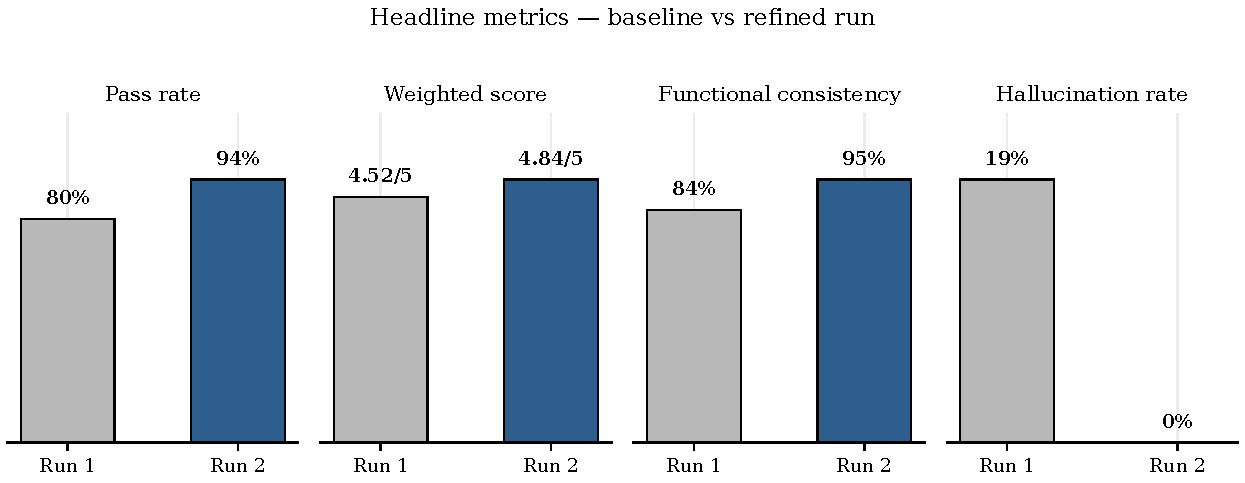
\includegraphics[width=\textwidth]{figures/metrics_dashboard.pdf}
    \caption{Headline metrics. Run~1 (grey) vs Run~2 (blue). Every dimension improves; hallucination rate drops to zero.}
    \label{fig:dashboard}
\end{figure}

Pass rate: 80\% $\to$ 94\%. Weighted score: 4.52 $\to$ 4.84 out of 5.0. Functional consistency: 84\% $\to$ 95\%. Hallucination rate: 19\% $\to$ \textbf{0\%}. The refined agent fabricates nothing across 81 runs.

\begin{tcolorbox}[colback=scblue!4, colframe=scblue!60, fonttitle=\bfseries, title=Result,
    boxrule=0.5pt, arc=2pt, left=6pt, right=6pt, top=3pt, bottom=3pt]
Across 81 refined evaluations: \textbf{94\% pass rate}, \textbf{4.84/5.0} weighted score, \textbf{zero fabricated data}.
\end{tcolorbox}

\section{Refinement Cycle}
\label{sec:finetuning}

Three changes between the two passes account for the improvement.

\textbf{Ground-truth recalibration.} Five scenarios in Run~1 passed at 0\% despite high underlying scores. Inspection showed the ground truths listed scenario-only identifiers while the agent correctly used the full dataset, and the judge flagged the extensions as hallucinations. Four were rewritten to focus on answer shape; one had a single over-strict critical fact demoted to important.

\textbf{Judge prompt revision.} An explicit rule was added: identifiers matching the domain patterns are not hallucinations unless they contradict the ground truth. The \texttt{hallucination} failure category is now reserved for genuine fabrication (names outside the domain, impossible values, contradictions).

\textbf{Agent prompt revision.} A \emph{Rules to Avoid Mistakes} section was added to the agent's system prompt: never invent identifiers, distinguish active from historical data, list all matching items, compute metrics over the full result set, respect the critical business rules on cold chain and reorder points.

\section{By Complexity Level}

\begin{figure}[H]
    \centering
    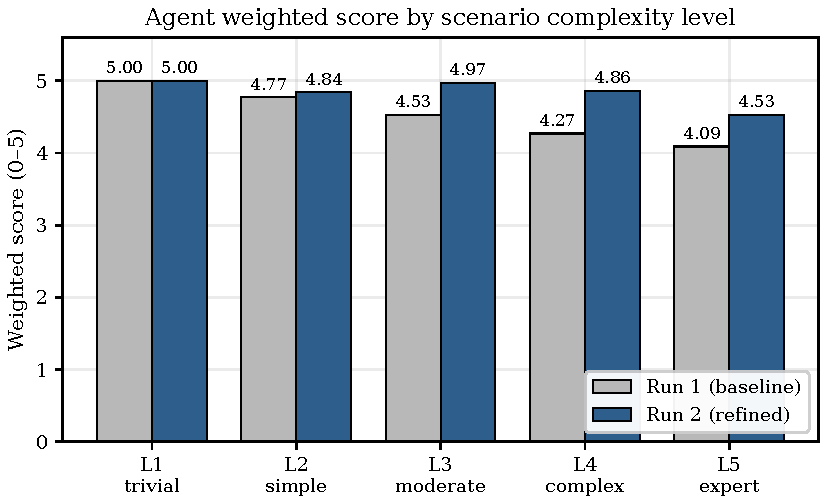
\includegraphics[width=0.92\textwidth]{figures/score_by_level.pdf}
    \caption{Weighted score by complexity level.}
    \label{fig:score_level}
\end{figure}

Accuracy decreases with complexity, as expected, but flattens in Run~2. L1 stays at 5.0. L3 rises 4.53 $\to$ 4.97. \textbf{L4 rises 4.27 $\to$ 4.86 and passes at 100\%}---the canonical cross-system diagnostics all succeed. L5 rises 4.09 $\to$ 4.53 and remains the hardest level.

\section{By Use Case}

\begin{figure}[H]
    \centering
    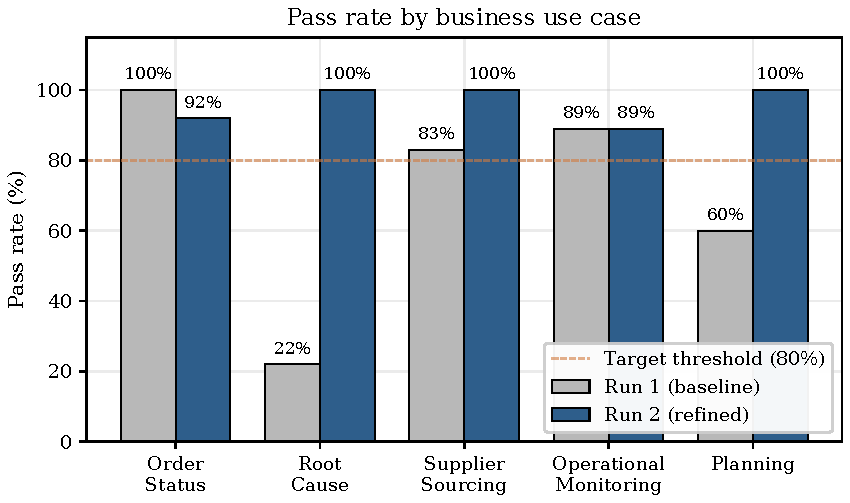
\includegraphics[width=0.92\textwidth]{figures/pass_rate_by_uc.pdf}
    \caption{Pass rate by business use case.}
    \label{fig:pass_uc}
\end{figure}

UC-2 (Root Cause) rises from 22\% to 100\%---the largest shift. UC-3 and UC-5 also reach 100\%. UC-4 stays at 89\%. UC-1 regresses marginally (100\% $\to$ 92\%) because of one partial L2 answer, which does not affect the aggregate.

\section{Failure Taxonomy}

\begin{figure}[H]
    \centering
    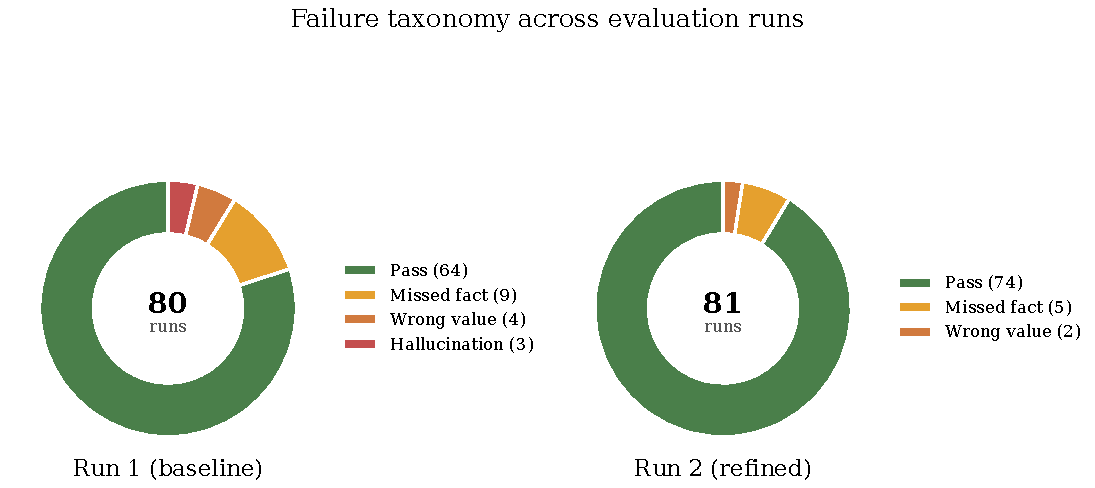
\includegraphics[width=\textwidth]{figures/failure_taxonomy.pdf}
    \caption{Failure taxonomy for both passes.}
    \label{fig:failures}
\end{figure}

\texttt{hallucination} falls from 4\% to 0\%, \texttt{wrong\_value} from 5\% to 2\%, \texttt{missed\_fact} from 11\% to 6\%. The zero-hallucination outcome is the combined effect of the agent rule (never invent) and the judge rule (no false positive on legitimate extensions).

\section{Resolution Time}

\begin{figure}[H]
    \centering
    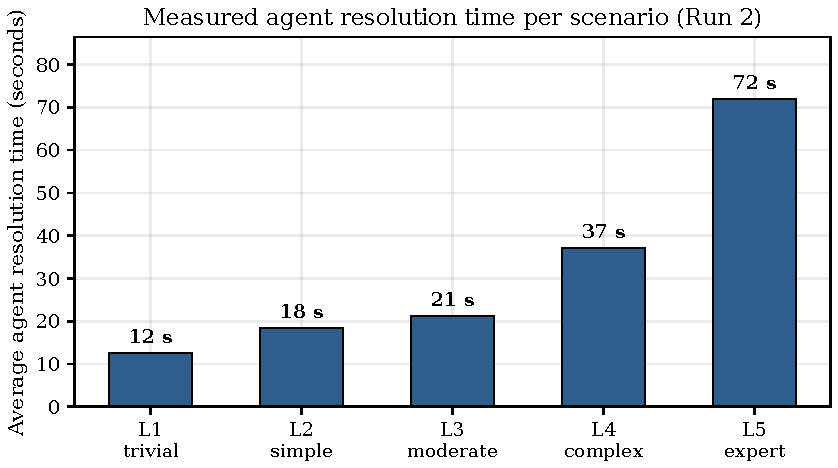
\includegraphics[width=\textwidth]{figures/time_savings.pdf}
    \caption{Measured agent resolution time per complexity level (Run~2).}
    \label{fig:time}
\end{figure}

Measured averages per scenario: L1 $\approx$ 13\,s, L2 $\approx$ 18\,s, L3 $\approx$ 21\,s, L4 $\approx$ 37\,s, L5 $\approx$ 72\,s. Across the 81 Run~2 evaluations the agent spent 43.5\,min in total, averaging about 32\,s per run.

\section{Cross-System Coverage}

\begin{figure}[H]
    \centering
    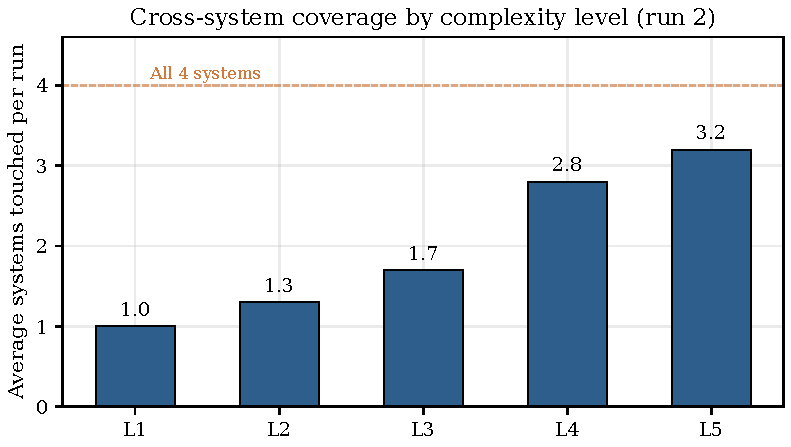
\includegraphics[width=0.85\textwidth]{figures/systems_touched.pdf}
    \caption{Average systems touched per run, by level (Run~2).}
    \label{fig:coverage}
\end{figure}

L1 averages 1 system; L4 averages 2.8; L5 averages 3.2. The agent does chain across systems when the question requires it, and stays scoped when it does not.

\section{Qualitative Behaviour}

Three Run~2 responses illustrate behaviour that scalar metrics do not fully capture. On the carrier-mismatch diagnosis, the agent identifies the storage-type mismatch, references the \texttt{SHP-009} refrigeration failure as evidence, and lists refrigerated alternatives---a production-quality incident report. On the full product history, the agent chains six tool calls, computes a running stock balance from movements, produces an ASCII flow diagram, and ends with a two-sentence takeaway. On the fulfilment-feasibility question, it computes the 4-unit gap, compares the two refrigerated carriers, and proposes three options with trade-offs.
